%#########################################

% author: S. Parisa Daj.
% email: s.dajkhosh@memphis.edu
% University of Memphis
% Sep 2021

%#########################################

\documentclass[12pt,oneside,geqno]{article}

\addtolength{\textheight}{120pt}
\oddsidemargin=-10pt
\topmargin=-.5in
\textwidth=6.5in
\pagestyle{empty}

% ######################## 	Packages
\usepackage{amssymb,latexsym,amsmath,amsthm}
\usepackage{amsfonts,raWFonts}
\usepackage{thmtools}
\usepackage{systeme}
\usepackage{mathtools}
\usepackage[usenames,dvipsnames]{color}
\usepackage{xcolor}
\usepackage{xfrac}
\usepackage{hyperref}
\usepackage[utf8]{inputenc}
\usepackage{enumerate}



\usepackage{listings}
\usepackage{xcolor}

\usepackage{graphicx}
\usepackage{caption}
\usepackage{subcaption}

% ######################## 	Colors
\definecolor{codegreen}{rgb}{0,0.6,0}
\definecolor{codegray}{rgb}{0.5,0.5,0.5}
\definecolor{codepurple}{rgb}{0.58,0,0.82}
\definecolor{backcolour}{rgb}{0.97,0.97,0.95}

% ######################## 	Style
\lstdefinestyle{mystyle}{
	backgroundcolor=\color{backcolour},   
	commentstyle=\color{codegreen},
	keywordstyle=\color{magenta},
	numberstyle=\tiny\color{codegray},
	stringstyle=\color{codepurple},
	basicstyle=\ttfamily\footnotesize,
	breakatwhitespace=false,         
	breaklines=true,                 
	captionpos=b,                    
	keepspaces=true,                 
	numbers=left,                    
	numbersep=5pt,                  
	showspaces=false,                
	showstringspaces=false,
	showtabs=false,                  
	tabsize=2
}

\lstset{style=mystyle}

\declaretheoremstyle[
headfont=\color{blue}\normalfont\bfseries,
notefont=\bfseries, 
notebraces={}{},
%bodyfont=\color{red}\normalfont\itshape,
bodyfont=\normalfont,%\itshape,
%headformat=\NUMBER.~\NAME\NOTE
headformat=\NAME\NOTE
]{colorejercicio}

\declaretheorem[
%numbered=no,
style=colorejercicio,
name=Problem
]{Problem}

% ######################## 	Document
\begin{document}
	
	\begin{center}
		{\LARGE EECE 8740-Neural Networks HW \#4}% Title
		\vspace*{1\baselineskip}   
		
		\scshape % Small caps
		\color{red}{(Solutions)}\\
		%  
		\vspace*{1\baselineskip}
		\color{black}University of Memphis\\[\baselineskip]
		%
		\vspace*{5\baselineskip} 
		
		Written by \\[\baselineskip]
		{\Large S. Parisa Daj.\par U00743495} \\
		(s.dajkhosh@memphis.edu)\\
		
		\vspace*{1\baselineskip}
		\today
	\end{center}
	%
	\clearpage
	
	
	\section{Introduction}
	The goal of this assignment is to translate English to French using three different models. All three models are stacked two-layer RNN, stacked two-layer LSTM, and stacked two-layer GRU. The dataset consists of 137860 English sentences, each having a French translation as well. To perform the task, a portion of \%80 of these sentences are trained by the model. Then, it is evaluated on the remaining \%20 sentences. However, to be able to train the model, the data needs to be pre-processed. The first part of pre-processing the data is tokenizing as the data includes words, but the model accepts arrays of numbers. The outputs of the models are also numbers. Thus, the outputs need to be converted to the text again.
	
	\section{Methodology and Deep Learning Architecture}
	The code is accessible by \href{https://colab.research.google.com/drive/1D5zuU2iycZJFkAeJsVisMA7ne8joUwxD?usp=sharing}{this link} on Google Colaboratory using GPU. The data is downloaded from GitHub and uploaded to Google Colab from a local file. It was also possible to download them directly to Google Colab from GitHub. The codes for pre-processing and GRU were available as resources for the code. To tokenize, the "Tokenizer" object is utilized, also we are using the "pad\_sequences" function for padding. Both from Keras's pre-processing packages. 
	
	All three models take sequences of pre-processed words (sentences) as input.  The input is then passed to the model regarding the task and again passed to the same model so that we can build two-layer stacked models. the models are chosen from the Keras layers package including SimpleRNN, LSTM, GRU. they take the units number equal to the dimensionality of the output space (64 here). The parameter "return\_sequence" is selected to be true so that a sequence of words is received in output as a sentence. The rest of the parameters are chosen as default values for all three models. The number of epochs is 25, the batch size is 16, Adam is the optimizer and they all use sparse cross-entropy loss function. One fully connected layer with SoftMax activation function is added at the final stage to specify the number of classes which is equal to the French vocabulary size. The model architecture for each are presented as shown in tables \ref{t:rnn}, \ref{t:lstm}, and \ref{t:gru}.
	
	\begin{table}[h]
		\centering
		\begin{tabular}{|l|l|l|}
			\hline
			Layer (Type)                    & Output Shape        & Param \# \\ \hline
			input\_9 (InputLayer)           & {[}(None, 21, 1){]} & 0        \\ \hline
			simple\_rnn\_2 (SimpleRNN)      & (None, 21, 64)      & 4224     \\ \hline
			simple\_rnn\_3 (SimpleRNN)      & (None, 21, 64)      & 8256     \\ \hline
			time\_distributed\_6 (TimeDist) & (None, 21, 345)     & 22425    \\ \hline
			activation\_4 (Activation)      & (None, 21, 345)     & 0        \\ \hline
		\end{tabular}
		\caption{Stacked RNN Model Architecture}
		\label{t:rnn}
	\end{table}
	
	\begin{table}[h]
		\centering
		\begin{tabular}{|l|l|l|}
			\hline
			Layer (Type)                    & Output Shape        & Param \# \\ \hline
			input\_10 (InputLayer)           & {[}(None, 21, 1){]} & 0        \\ \hline
			lstm\_4 (LSTM)      & (None, 21, 64)      & 16896     \\ \hline
			lstm\_5 (LSTM)      & (None, 21, 64)      & 33024     \\ \hline
			time\_distributed\_7 (TimeDist) & (None, 21, 345)     & 22425    \\ \hline
			activation\_5 (Activation)      & (None, 21, 345)     & 0        \\ \hline
		\end{tabular}
		\caption{Stacked LSTM Model Architecture}
		\label{t:lstm}
	\end{table}
	
	\begin{table}[h]
		\centering
		\begin{tabular}{|l|l|l|}
			\hline
			Layer (Type)                    & Output Shape        & Param \# \\ \hline
			input\_11 (InputLayer)           & {[}(None, 21, 1){]} & 0        \\ \hline
			gru\_6 (GRU)      & (None, 21, 64)      & 12864     \\ \hline
			gru\_7 (GRU)      & (None, 21, 64)      & 24960     \\ \hline
			time\_distributed\_8 (TimeDist) & (None, 21, 345)     & 22425    \\ \hline
			activation\_6 (Activation)      & (None, 21, 345)     & 0        \\ \hline
		\end{tabular}
		\caption{Stacked RNN Model Architecture}
		\label{t:gru}
	\end{table}
	
	To return the network's results to the text there is a "logits\_to\_text" function provided by the source. Furthermore, as one of the task's requirements, to select ten sentences to be translated by the trained model randomly, there is another function responsible to make the random choice. 
	\pagebreak
	
	\section{Experimental and Test Results}
	After training all three models, the results are impressive. With only 25 epochs, they all reach an accuracy above \%80. However, running each of them took about 1 hour with GPU. The specific results for each model is shown in table \ref{t:compare} and figures\ref{fig:rnn}, \ref{fig:lstm}, and \ref{fig:gru}. The results clearly show that LSTM is outperforming the two other models, and the lowest accuracy is for the simple RNN model, which was expected. We can also see that the higher the accuracy is, there are more parameters for the neural network to learn. Therefore, more time is utilized. Clearly, there is a trade-off depending on our limitations to prefer the model with higher accuracy or the one which takes less time and computation to run. 
	
	\begin{table}[h]
		\begin{tabular}{|l|l|l|l|}
			\hline
			Model        & Validation Accuracy (\%) & Trainable Parameters \# & Training Time (s) \\ \hline
			Stacked RNN  & 80.74                    & 34,905                  & 2501              \\ \hline
			Stacked LSTM & 84.35                    & 72,345                  & 4094              \\ \hline
			Stacked GRU  & 82.30                    & 60,249                  & 3574              \\ \hline
		\end{tabular}
		\caption{Compare logs for the three stacked RNN, LSTM, and GRU models}
		\label{t:compare}
	\end{table}
	
	\begin{figure}
		\centering
		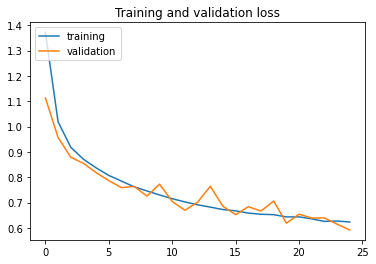
\includegraphics[width=\textwidth]{../figs/stacked_rnn_results.png}
		\label{fig:rnn}
		\caption{Accuracy and loss graph for stacked RNN}
	\end{figure}
	\begin{figure}
		\centering
		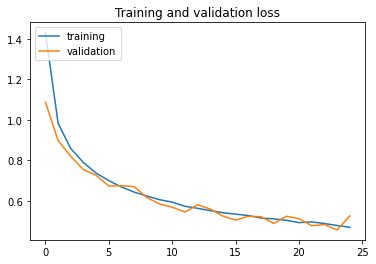
\includegraphics[width=\textwidth]{../figs/stacked_lstm_results.png}
		\label{fig:lstm}
		\caption{Accuracy and loss graph for stacked LSTM}
	\end{figure}
	\begin{figure}
		\centering
		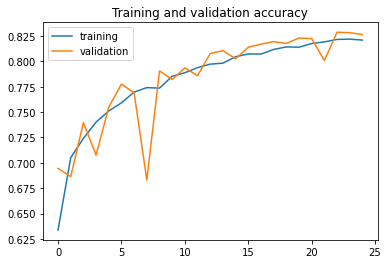
\includegraphics[width=\textwidth]{../figs/stacked_gru_results.png}
		\label{fig:gru}
		\caption{Accuracy and loss graph for stacked GRU}
	\end{figure}
	
	Ten random sentences are translated using each model. The results are shown as follows: 
	\pagebreak
	\subsection{Stacked RNN}
	1 : sentence num 54331\\
	france is sometimes wet during october , and it is never relaxing in february .\\
	la france est parfois humide en octobre et il est jamais humide en février\\\\
	
	2 : sentence num 32563\\
	paris is sometimes freezing during january , and it is cold in july .\\
	paris est parfois agréable gel en janvier et il est chaud en juillet \\\\
	
	3 : sentence num 59266\\
	paris is beautiful during fall , but it is sometimes busy in september .\\
	paris est agréable en juin mais il est parfois occupé en juillet \\\\
	
	4 : sentence num 24576\\
	paris is usually cold during october , and it is usually chilly in june .\\
	paris est généralement froid en octobre et il est généralement froid en juin \\\\
	
	5 : sentence num 92230\\
	paris is sometimes wet during november , but it is never hot in may .\\
	paris est parfois humide en mois de novembre mais il est jamais mai en mai \\\\
	
	6 : sentence num 80902\\
	your favorite fruit is the strawberry , but my favorite is the apple.\\
	votre fruit préféré est la fraise mais mon préféré est la pomme \\\\
	
	7 : sentence num 24866\\
	the united states is rainy during spring , but it is sometimes dry in february .\\
	les états unis est pluvieux au l'automne mais il est parfois merveilleux en février \\\\
	
	8 : sentence num 124368\\
	she likes mangoes and oranges .\\
	elle aime les mangues et les oranges \\\\
	
	9 : sentence num 84704\\
	they dislike bananas , grapefruit , and limes .\\
	ils n'aiment les bananes le pamplemousse et les citrons\\\\
	
	10 : sentence num 126091\\
	china is never dry during april , and it is sometimes busy in july .\\
	chine est jamais jamais sec avril et il est parfois occupé en juillet \\\\
	
	\subsection{Stacked LSTM}
	1 : sentence num 59885\\
	india is sometimes wet during spring , but it is rainy in fall .\\
	l' inde est parfois humide au printemps mais il est froid à l' automne \\\\
	
	2 : sentence num 92618\\
	california is never pleasant during winter , and it is sometimes hot in september .\\
	californie est jamais agréable le gel pendant l' hiver et il est parfois calme en septembre \\\\
	
	3 : sentence num 105663\\
	the united states is usually warm during august .\\
	0	la états unis est généralement chaud en mois mois août août \\\\
	
	4 : sentence num 125950\\
	the united states is never wet during march , and it is pleasant in october .\\
	la états unis est jamais doux en l' et il est il en octobre \\\\
	
	5 : sentence num 41756\\
	he dislikes grapefruit , apples , and strawberries .\\
	il aime pas pamplemousse pamplemousse les mangues et poires \\\\
	
	6 : sentence num 69113\\
	california is usually busy during summer , and it is relaxing in june .\\
	californie est généralement sec en l' été et il est relaxant en juin \\\\
	
	7 : sentence num 50481\\
	she likes pears , peaches , and grapefruit .\\
	elle aime les poires les pêches et le pamplemousse \\\\
	
	8 : sentence num 115390\\
	new jersey is never warm during april , but it is never mild in winter .\\
	new jersey est jamais chaud neige avril mais il est jamais doux en hiver \\\\
	
	9 : sentence num 39249\\
	france is sometimes pleasant during summer , but it is usually mild in spring .\\
	la france est parfois agréable gel pendant l' mais mais il est généralement pluvieux au \\\\
	
	10 : sentence num 91047\\
	new jersey is chilly during july , but it is wet in fall .\\
	new jersey est froid en juillet mais il est doux en l' automne \\\\
	
	\subsection{Stacked GRU}
	1 : sentence num 47020\\
	china is cold during spring , and it is never mild in march .\\
	chine est froid en printemps et il est jamais doux en l' \\\\
	
	2 : sentence num 64270\\
	the united states is never wonderful during fall , but it is usually pleasant in february .\\
	la états unis est jamais merveilleux sec à cours automne mais il mais généralement en en \\\\
	
	3 : sentence num 103291\\
	they like mangoes , strawberries , and lemons.\\
	ils aiment les les les les et les citrons \\\\
	
	4 : sentence num 13508\\
	the orange is her most loved fruit , but the banana is their most loved .\\
	la est est son fruit le plus aimé mais la chaux est plus plus aimé \\\\
	
	5 : sentence num 17116\\
	the strawberry is his least liked fruit , but the grape is our least liked .\\
	la fraise est son fruit aimé des fruits mais le raisin est notre aimé aimé \\\\
	
	6 : sentence num 38359\\
	my least liked fruit is the pear , but your least liked is the lemon .\\
	mon fruit est moins aimé la poire mais votre moins aimé est la citron \\\\
	
	7 : sentence num 28578\\
	china is usually wet during may , and it is pleasant in june .\\
	chine est généralement humide en au mois de mai et il est agréable en juin \\\\
	
	8 : sentence num 86796\\
	you dislike strawberries , grapefruit , and limes .\\
	vous n'aimez pas poires poires le pamplemousse les citrons \\\\
	
	9 : sentence num 17381\\
	the pear is their least favorite fruit , but the lime is your least favorite .\\
	la poire est leur fruit préféré moins mais la chaux est votre préféré moins \\\\
	
	10 : sentence num 76045\\
	new jersey is usually hot during october , and it is sometimes pleasant in may .\\
	new jersey est généralement chaud en octobre et il est parfois agréable en mai\\\\
	
	
	\section{Conclusion}
	The point of this assignment was being able to implement three different stacked models to translate English words to French: 1- RNN, 2- LSTM, and 3- GRU. Afterward, we could provide some random translations from each model and compare these three models together. All models reach an acceptable accuracy. However, LSTM with more parameters takes more time but comes up with the highest accuracy. In contrast, RNN has the fewest number of trainable parameters, it takes less time to run, but the accuracy is the lowest. Looking at the sample translations, it seems that even a small improvement in the accuracy results in a more acceptable translation. Thus, if there is enough time and resources, LSTM is highly recommended. Moreover, looking at the accuracy figure for all three models, the training plot moves very closely with the validation plot. Meaning that the model is not memorizing the training data, and there is still a place to increase the number of iterations. Then, we will definitely face higher validation accuracies.
	
	%
	%\bibliography{bibfile} 
	%\bibliographystyle{ieeetr}
	
\end{document}